\documentclass[10pt,a4paper,twocolumn]{article}
\usepackage[margin=0.6in]{geometry}
\usepackage{graphicx}
\usepackage{caption}
\usepackage{subcaption}
\usepackage{amsmath}
\usepackage{listings}
\usepackage{xcolor}
\usepackage{bookmark}
\usepackage{hyperref}
\usepackage{setspace}
\setstretch{0.9}

% Adjust column spacing
\setlength{\columnsep}{25pt}
\setlength{\columnseprule}{0.8pt}

% Adjust figure spacing
\setlength{\floatsep}{8pt plus 2pt minus 2pt}
\setlength{\textfloatsep}{10pt plus 2pt minus 4pt}
\setlength{\intextsep}{8pt plus 2pt minus 2pt}
% Define custom colors for code style
\definecolor{codegreen}{rgb}{0,0.6,0}
\definecolor{codegray}{rgb}{0.5,0.5,0.5}
\definecolor{codepurple}{rgb}{0.58,0,0.82}
\definecolor{backcolour}{rgb}{0.95,0.95,0.92}

\lstdefinestyle{mystyle}{
    backgroundcolor=\color{backcolour},
    commentstyle=\color{codegreen},
    keywordstyle=\color{magenta},
    numberstyle=\tiny\color{codegray},
    stringstyle=\color{codepurple},
    basicstyle=\ttfamily\scriptsize,
    breakatwhitespace=false,
    breaklines=true,
    captionpos=b,
    keepspaces=true,
    numbers=left,
    numbersep=3pt,
    showspaces=false,
    showstringspaces=false,
    showtabs=false,
    tabsize=2,
    frame=single,
    rulecolor=\color{black},
    title=\lstname,
    aboveskip=8pt,
    belowskip=8pt
}
\lstset{style=mystyle}
\usepackage{float}

\lstset{breaklines=true, basicstyle=\ttfamily\scriptsize, columns=fullflexible}


\hypersetup{colorlinks=true,linkcolor=blue,urlcolor=blue,citecolor=blue}

\title{EN3160 Assignment 02 Report}
\author{T.N. Kodithuwakku \\ Index: 220325X \\ \href{https://github.com/TNKodi/EN3160--A02.git}{MY GitHub Repo}}
\date{\today}

\begin{document}
\maketitle
\begin{@twocolumnfalse}

\vspace{1pt}
\end{@twocolumnfalse}

%--------------------

\section{Question 1: LoG-based Blob Detection}



\subsection*{LoG-based Blob Detection Method}
The Laplacian of Gaussian (LoG) method detects blobs by finding scale-space extrema. The LoG operator combines Gaussian smoothing at various scales ($\sigma$) with the Laplacian operator to highlight blob-like structures. Blobs appear as local maxima in the scale-space representation, where both spatial location and scale are considered.

\vspace{2pt}
\begin{lstlisting}[language=Python, style=mystyle]
def laplacian_of_gaussian(image, sigma):
    """Apply Laplacian of Gaussian at a specific scale."""
    img_float = image.astype(np.float32)
    gaussian = cv.GaussianBlur(img_float, (0, 0), sigma)
    laplacian = cv.Laplacian(gaussian, cv.CV_32F, ksize=3)
    # Normalize by sigma^2 for scale invariance
    return laplacian * (sigma ** 2)

def blob_detection_log(image):
    """Detect blobs using LoG at multiple scales."""
    sigma_min, sigma_max, num_scales = 1, 30, 10
    sigmas = np.logspace(np.log10(sigma_min), np.log10(sigma_max), num_scales)
    log_responses = []
    for sigma in sigmas:
        log_response = laplacian_of_gaussian(image, sigma)
        log_responses.append(log_response)
    return np.stack(log_responses, axis=2), sigmas

\end{lstlisting}

\vspace{2pt}

\subsection*{LoG Responses at Different $\sigma$ Values}
The LoG operator is applied at multiple scales to detect blobs of different sizes. The response intensity indicates the likelihood of blob presence at each scale.

\vspace{1pt}
\begin{lstlisting}[language=Python, style=mystyle]
# Generate LoG responses at test sigma values
sigma_test = [1, 2, 5, 10, 20]
fig, axes = plt.subplots(1, 5, figsize=(20, 4))
for i, sigma in enumerate(sigma_test):
    log_response = laplacian_of_gaussian(gray, sigma)
    axes[i].imshow(log_response, cmap='RdBu_r')
    axes[i].set_title(f'LoG Response ($\sigma$={sigma})')
    axes[i].axis('off')
plt.tight_layout()
plt.savefig('fig/Q1_log_responses.png', dpi=200, bbox_inches='tight')
\end{lstlisting}

\begin{figure}[H]
\centering
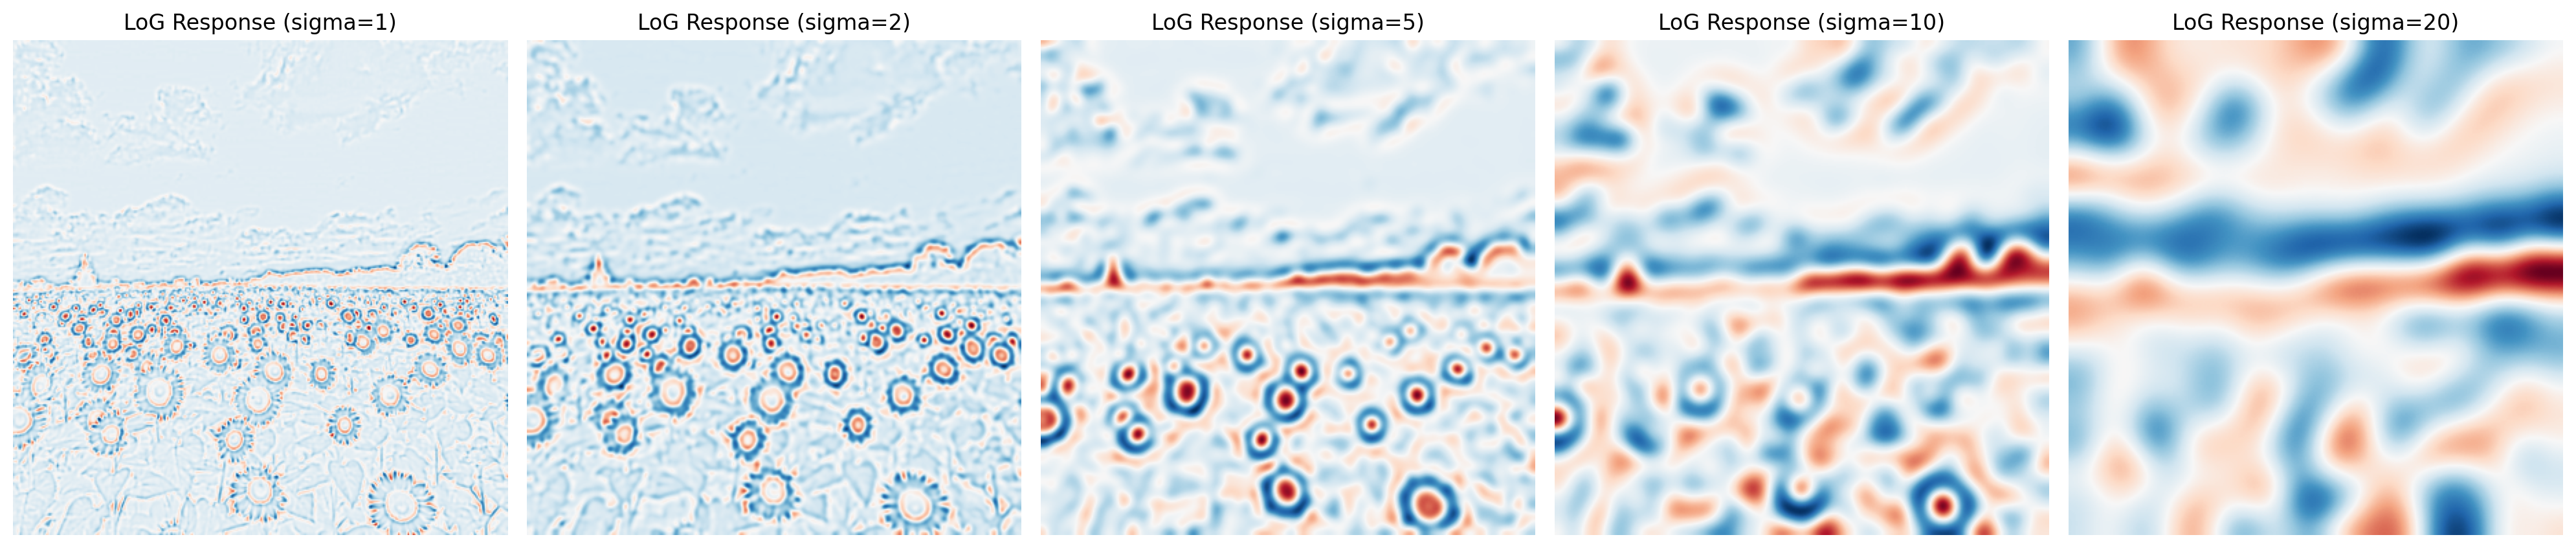
\includegraphics[width=0.95\columnwidth]{fig/Q1_log_responses.png}
\caption{LoG responses at different $\sigma$ values showing blob detection at multiple scales.}
\label{fig:q1_log}
\end{figure}


\subsection*{Blob Detection Results}
The complete blob detection pipeline is applied to detect and localize circular structures in the sunflower field.

\vspace{2pt}
\begin{lstlisting}[language=Python, style=mystyle]
log_response_stack, sigmas = blob_detection_log(gray)
blobs = find_scale_space_extrema(log_response_stack, sigmas, threshold=99)
filtered_blobs = non_maximum_suppression(blobs, overlap_threshold=0.5)
largest_circles = sorted(filtered_blobs, key=lambda b: b[4], reverse=True)[:10]
\end{lstlisting}

\vspace{1pt}
    \textbf{Key Results:}
\begin{itemize}
    \item \textbf{Largest Circle:} Center (285, 359), $\sigma=9.65$, radius=13.65 pixels
    \item \textbf{Sigma Range Used:} 1.00 to 30.00 (10 logarithmically spaced values)
    \item \textbf{Sigma Values:} [1.00, 1.46, 2.13, 3.11, 4.53, 6.62, 9.65, 14.07, 20.52, 30.00]
    \item \textbf{Total Detections:} 291 circles after non-maximum suppression
    \item \textbf{Radius Range:} 1.41 to 13.65 pixels (mean: 2.86 pixels)
\end{itemize}

\vspace{2pt}

\begin{figure}[H]
\centering
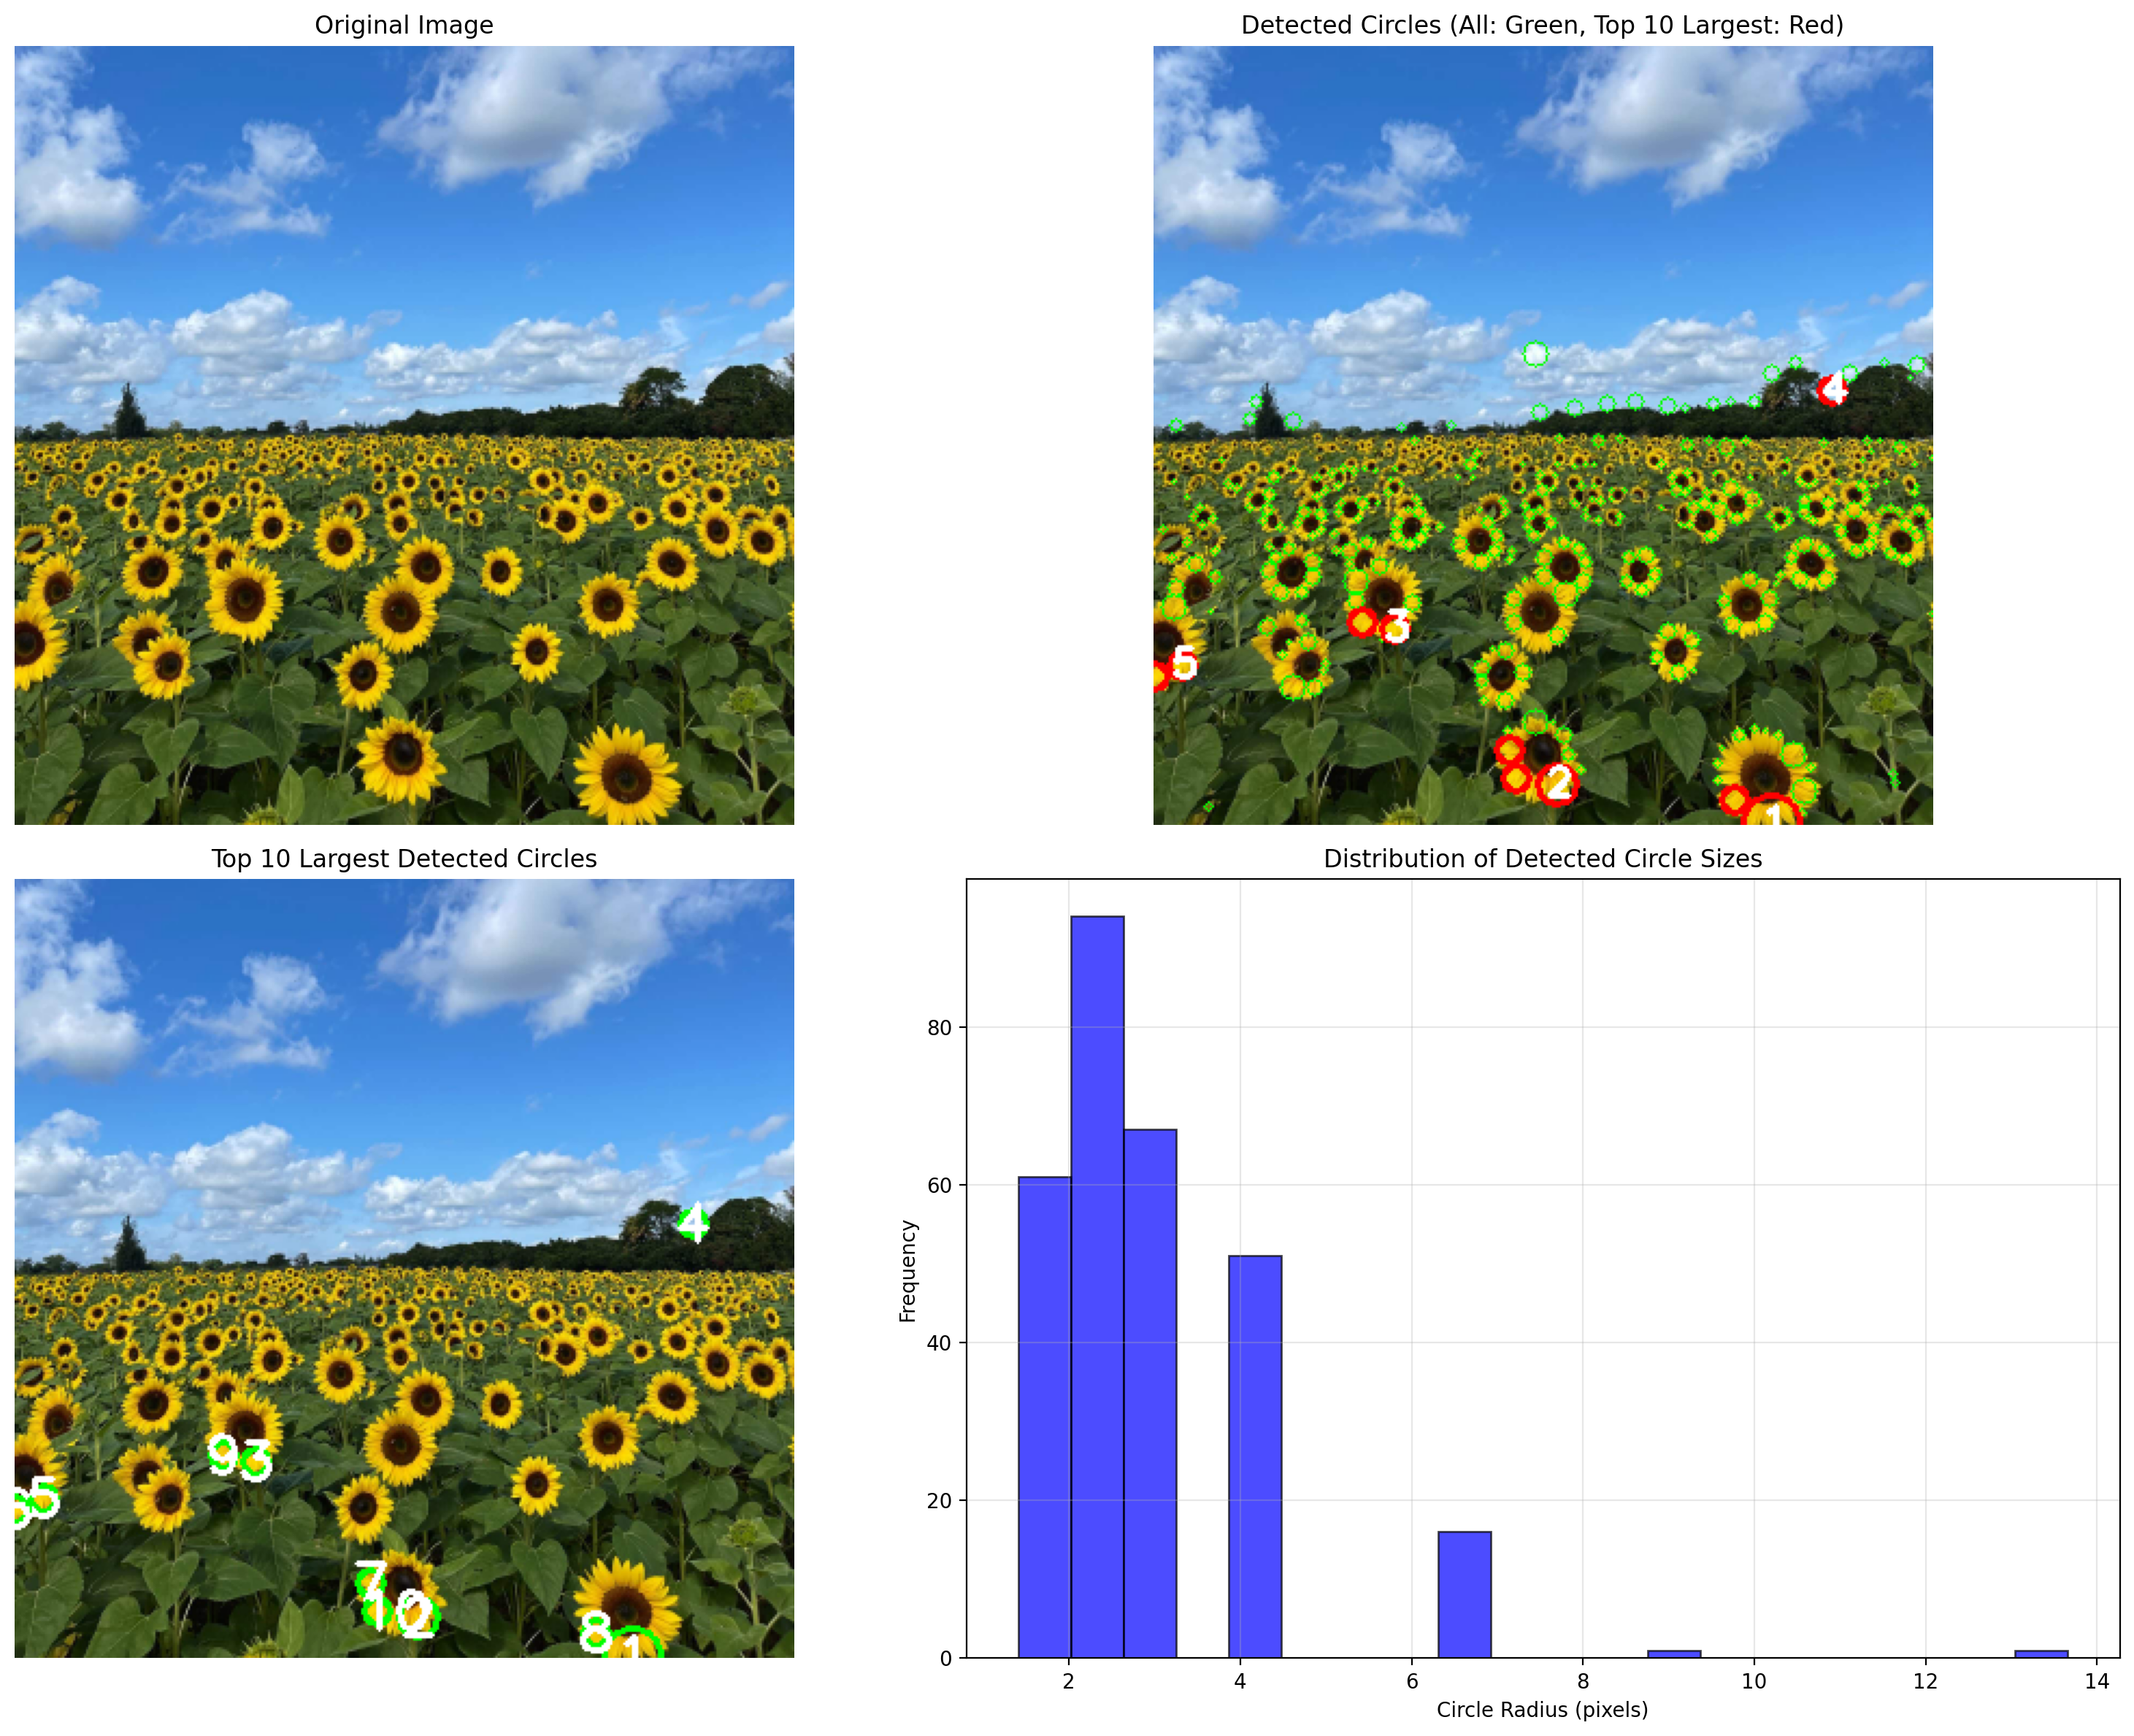
\includegraphics[width=0.95\columnwidth]{fig/Q1_detected_circles_and_hist.png}
\caption{Detected circles (green: all detections; red: top-10 largest) and radius histogram.}
\label{fig:q1_detected}
\end{figure}


%--------------------

\section{Question 2: RANSAC for Line and Circle}

\subsection*{(a) RANSAC Line and Circle Functions}
\textbf{Answer:} The following functions implement robust line and circle fitting using RANSAC. The line is fitted using total least squares, and the circle is fitted using nonlinear least squares. RANSAC iteratively samples minimal sets, fits a model, and counts inliers.

\begin{lstlisting}[language=Python, style=mystyle]
def fit_line_total_least_squares(points):
    mean = np.mean(points, axis=0)
    centered = points - mean
    U, S, Vt = np.linalg.svd(centered)
    a, b = Vt[-1]
    norm = np.sqrt(a**2 + b**2)
    a, b = a/norm, b/norm
    d = -np.dot(mean, [a, b])
    return a, b, d

def line_distance(a, b, d, points):
    return np.abs(a*points[:,0] + b*points[:,1] + d)

def ransac_line(X, threshold=1.5, min_inliers=30, max_trials=200):
    best_inliers = []
    best_params = None
    rng = np.random.default_rng()
    for _ in range(max_trials):
        sample_idx = rng.choice(len(X), 2, replace=False)
        sample = X[sample_idx]
        a, b, d = fit_line_total_least_squares(sample)
        distances = line_distance(a, b, d, X)
        inliers = np.where(distances < threshold)[0]
        if len(inliers) > len(best_inliers) and len(inliers) >= min_inliers:
            best_inliers = inliers
            best_params = (a, b, d)
    if best_params is not None:
        a, b, d = fit_line_total_least_squares(X[best_inliers])
        return (a, b, d), best_inliers
    else:
        return None, []

def fit_circle_least_squares(points):
    x_m, y_m = np.mean(points, axis=0)
    def calc_R(xc, yc):
        return np.sqrt((points[:,0]-xc)**2 + (points[:,1]-yc)**2)
    def cost(params):
        xc, yc, r = params
        return np.sum((calc_R(xc, yc) - r)**2)
    r0 = np.mean(calc_R(x_m, y_m))
    res = minimize(cost, [x_m, y_m, r0], method='Powell')
    xc, yc, r = res.x
    return xc, yc, r

def circle_distance(xc, yc, r, points):
    return np.abs(np.sqrt((points[:,0]-xc)**2 + (points[:,1]-yc)**2) - r)

def ransac_circle(X, threshold=0.5, min_inliers=30, max_trials=200):
    best_inliers = []
    best_params = None
    rng = np.random.default_rng()
    for _ in range(max_trials):
        sample_idx = rng.choice(len(X), 3, replace=False)
        sample = X[sample_idx]
        xc, yc, r = fit_circle_least_squares(sample)
        distances = circle_distance(xc, yc, r, X)
        inliers = np.where(distances < threshold)[0]
        if len(inliers) > len(best_inliers) and len(inliers) >= min_inliers:
            best_inliers = inliers
            best_params = (xc, yc, r)
    if best_params is not None:
        xc, yc, r = fit_circle_least_squares(X[best_inliers])
        return (xc, yc, r), best_inliers
    else:
        return None, []
\end{lstlisting}

\subsection*{(c) RANSAC Results}
\textbf{Answer:} RANSAC is first used to fit a line to the data, identifying inliers. These inliers are removed, 
and RANSAC is then used to fit a circle to the remaining points.
 The results show the effectiveness of RANSAC in separating and fitting both
  geometric shapes, even in the presence of noise and outliers.
\subsubsection{RANSAC Line fitting}
\begin{lstlisting}[language=Python, style=mystyle]
line_params, line_inliers = ransac_line(X, threshold=1.0, min_inliers=30, max_trials=500)
X_remnant = np.delete(X, line_inliers, axis=0)
circle_params, circle_inliers = ransac_circle(X_remnant, threshold=1.0, min_inliers=30, max_trials=500)
# Visualization and statistics (see notebook for full code)
\end{lstlisting}

\noindent\textbf{Reported Results (from execution):}
\begin{itemize}
    \item Line inliers: \textbf{47}
    \item Line parameters: $a=\mathbf{0.730}$, $b=\mathbf{0.684}$, $d=\mathbf{-1.667}$
\end{itemize}

\subsubsection{RANSAC Circle fitting}
\begin{lstlisting}[language=Python, style=mystyle]
circle_params, circle_inliers = ransac_circle(X_remnant, threshold=1.0, min_inliers=30, max_trials=500)
print(f"Circle inliers: {len(circle_inliers)}")
if circle_params is not None:
    print(f"Circle params: xc={circle_params[0]:.3f}, yc={circle_params[1]:.3f}, r={circle_params[2]:.3f}")
\end{lstlisting}

\begin{itemize}
    \item Circle inliers: \textbf{46}
    \item Circle parameters: $x_c=\mathbf{1.951}$, $y_c=\mathbf{3.138}$, $r=\mathbf{9.82}$
\end{itemize}

\begin{figure}[H]
\centering
\begin{subfigure}{0.48\columnwidth}
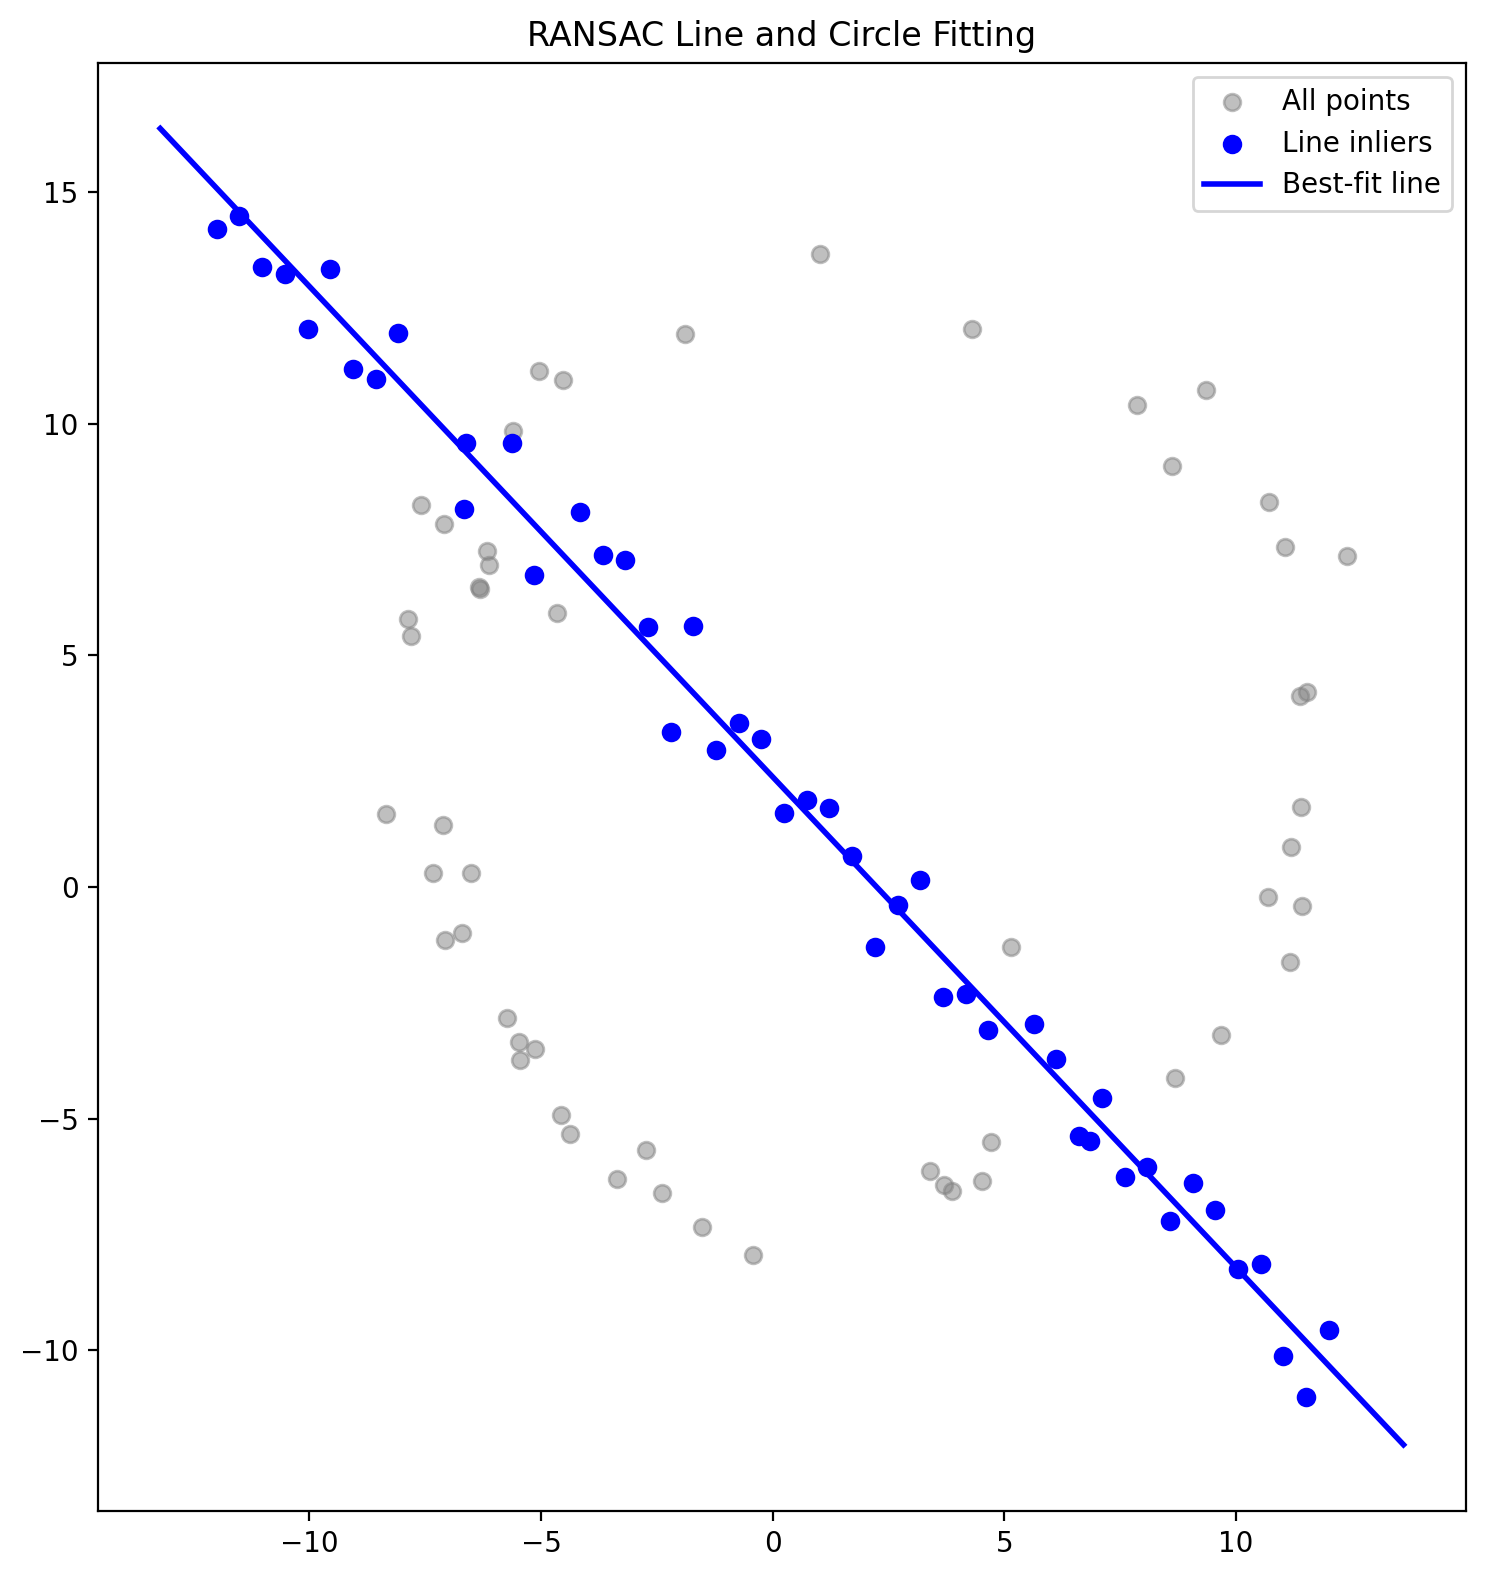
\includegraphics[width=\columnwidth]{fig/Q2_ransac_line.png}
\caption{RANSAC line fitting}
\end{subfigure}\hfill
\begin{subfigure}{0.48\columnwidth}
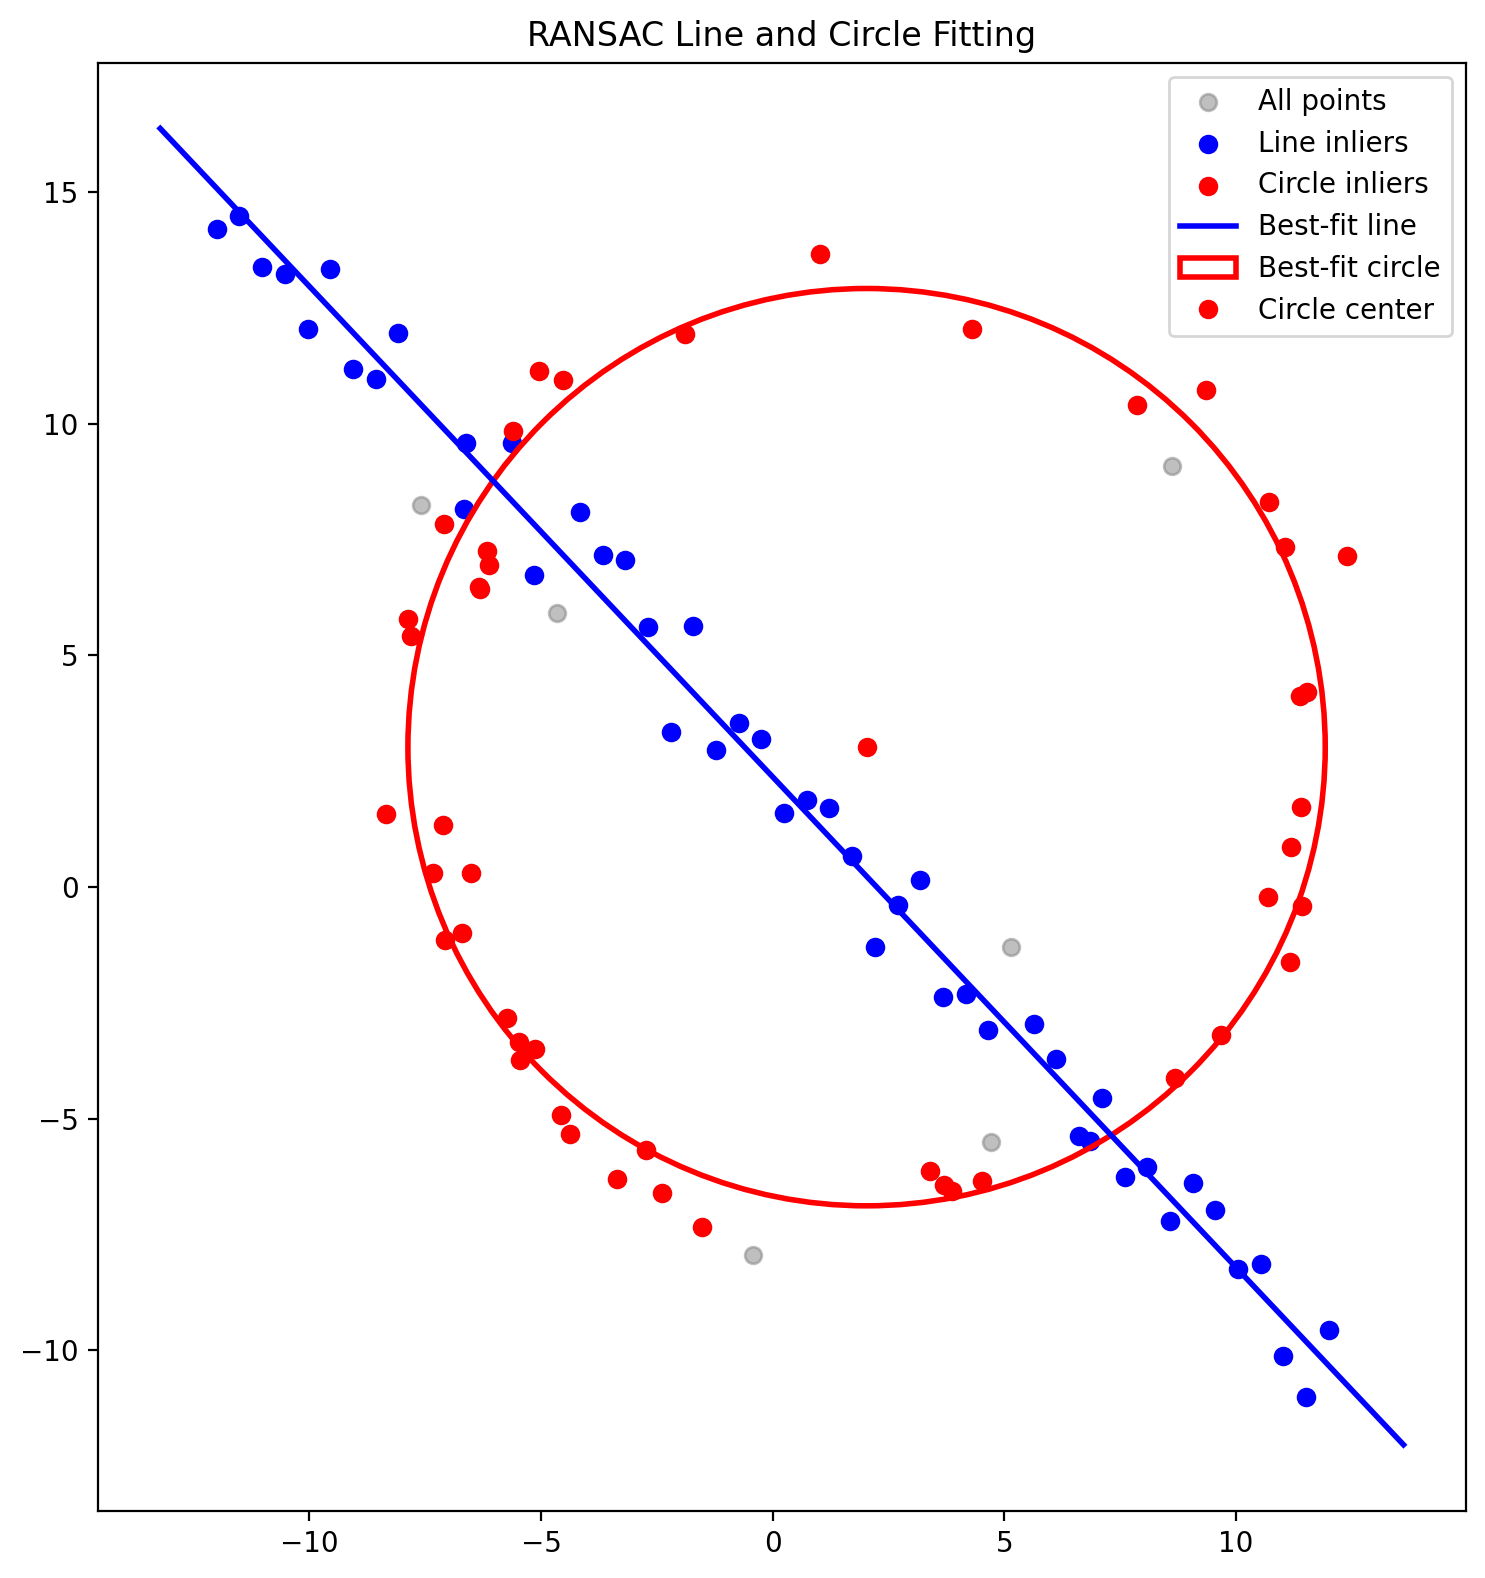
\includegraphics[width=\columnwidth]{fig/Q2_ransac_line_circle.png}
\caption{Line then circle}
\end{subfigure}
\caption{RANSAC: (a) Line inliers identified, (b) Circle fitted on remaining points.}
\label{fig:q2_results}
\end{figure}

\subsection*{Discussion: What if we fit the circle first?}
If we fit the circle first using RANSAC, the algorithm will try to find a circle that best fits the entire dataset, which contains both circle and line points. Since the line points do not conform to a circular shape, the fitted circle will be strongly influenced by these outliers. As a result, the estimated circle parameters will be less accurate, and the inlier count for the circle will be lower. After removing these (possibly incorrect) circle inliers, fitting a line to the remaining points will also be less robust. In summary, fitting the line first (when both shapes are present) is more robust because the line inliers are more easily separated from the mixed dataset, allowing for a cleaner subsequent circle fit.

%--------------------
\section{Question 3: Homography-Based Flag Overlay}


The process starts by selecting four corner points on the billboard where the flag will be placed. Using a mathematical technique called homography, the flag is stretched, rotated, and tilted so its corners align perfectly with those points, matching the billboard’s perspective. The flag is then warped to fit naturally onto the surface and blended with light transparency and feathered edges. This makes it appear as if the flag is truly part of the billboard, not just a digital overlay.

\vspace{4pt}
\noindent\textbf{Results on billboard}
\begin{figure}[H]
    \centering
    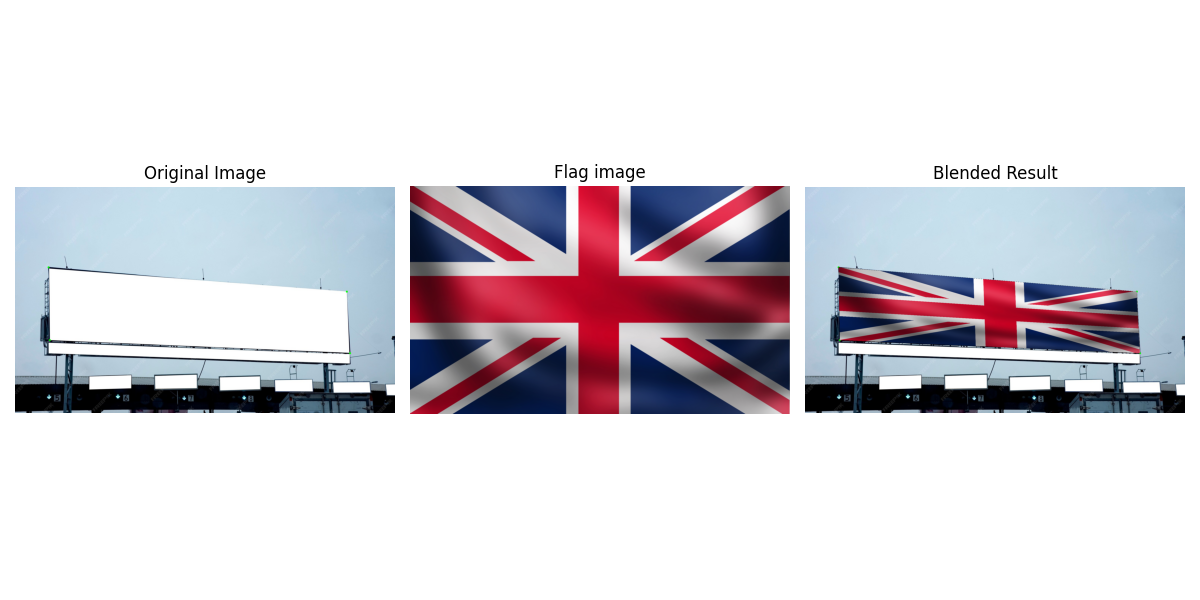
\includegraphics[width=0.95\columnwidth]{fig/Figure_1.png}
    \caption{Billboard overlay (Example 1): flag from 1.jpg overlaid onto 2.jpg using planar homography and alpha blending.}
    \label{fig:q3_billboard_ex1}
\end{figure}

\begin{figure}[H]
    \centering
    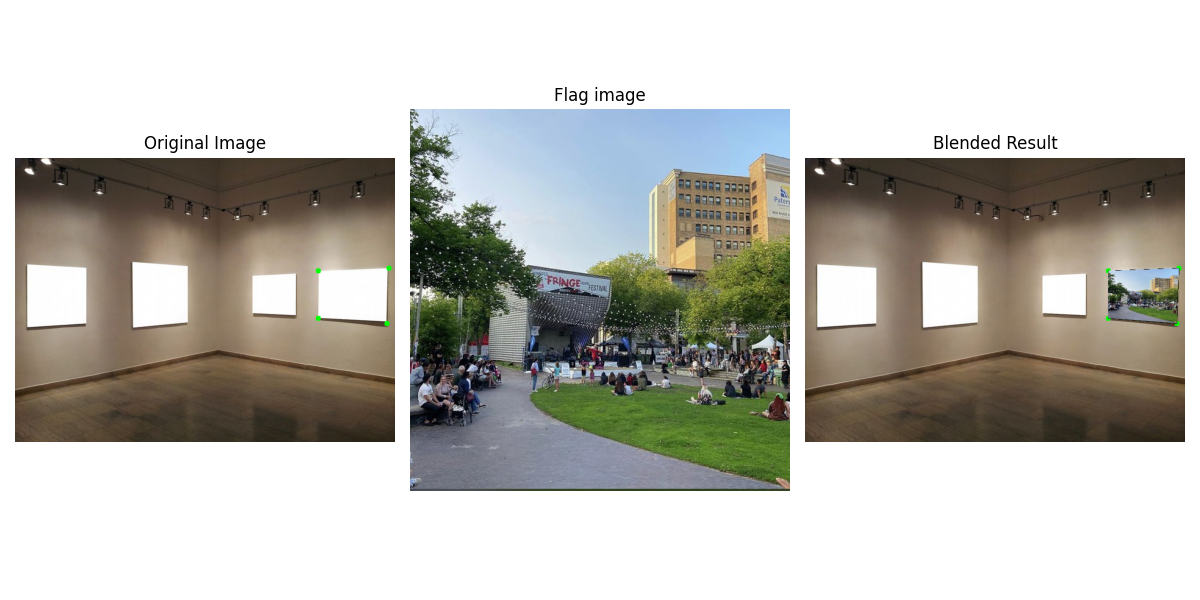
\includegraphics[width=0.95\columnwidth]{fig/Figure_2.png}
    \caption{Billboard overlay (Example 2) }
    \label{fig:q3_billboard_ex2}
\end{figure}
\subsubsection{Non Technical Review}
The selected images — a flag, billboard, art gallery, and outdoor festival — demonstrate how a simple 2D image can be realistically placed into various real-world settings. By choosing four corner points on a flat surface, applying a perspective transformation (homography), and blending the images, the flag appears naturally printed or displayed on each surface. This shows how digital overlays can be used creatively in environments like advertisements, gallery displays, or public events while maintaining a realistic visual effect.

%--------------------
\section{Question 4 SIFT Feature Matching and Homography}


\subsection*{4.1  Compute and match SIFT features between the two images.}

The SIFT algorithm detects distinctive keypoints in both images that remain stable under changes in scale, rotation, and lighting. It then extracts unique descriptors for each keypoint and matches them using distance-based methods such as Euclidean or FLANN matching. To improve reliability, Lowe’s ratio test filters out false matches, keeping only strong correspondences. These accurate feature matches are then visualized and used as the foundation for computing the homography and stitching the images together.

\vspace{2pt}
\begin{lstlisting}[language=Python, style=mystyle]
def get_features_and_matches(img1, img2,ratio=0.8):
    img1_g=cv.cvtColor(img1, cv.COLOR_BGR2GRAY)
    img2_g=cv.cvtColor(img2, cv.COLOR_BGR2GRAY)

    sift = cv.SIFT_create(nOctaveLayers=3, contrastThreshold=0.09, edgeThreshold=25, sigma=1)
    kp1, des1 = sift.detectAndCompute(img1_g, None)
    kp2, des2 = sift.detectAndCompute(img2_g, None)

    bf = cv.BFMatcher()
    matches = bf.knnMatch(des1, des2,k=2)
    best_matches = [m for m, n in matches if m.distance < ratio * n.distance]
    return best_matches, kp1, kp2
\end{lstlisting}

\begin{figure}[H]
    \centering
    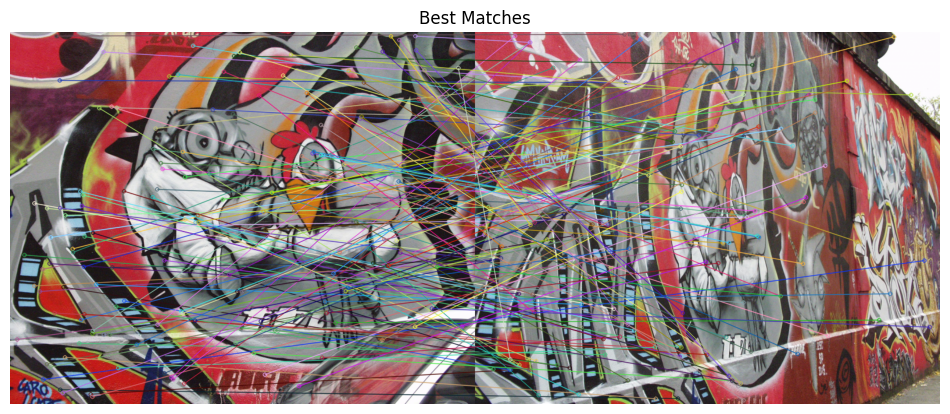
\includegraphics[width=0.95\columnwidth]{fig/4.1.png}
    \caption{Results for Q4.1: [Replace with a specific caption for 4.1.png]}
    \label{fig:q4_1}
\end{figure}


\subsection*{4.2 Homography Estimation and Inliers}

The next step is to estimate the homography matrix using RANSAC and the SIFT feature matches. The following function implements a custom RANSAC loop to robustly estimate the projective transformation (homography) and identify inliers:

\begin{lstlisting}[language=Python, style=mystyle]
def Htansform(best_matches, kp1, kp2):
    num_points=4
    threshold=8
    iters=500
    best_homography = None
    best_inliers = None
    binlier_count=0
    all_test_points = np.array([kp1[m.queryIdx].pt for m in best_matches])
    all_train_points = np.array([kp2[m.trainIdx].pt for m in best_matches])

    for i in range(iters):
        sample_indices = np.random.choice(len(best_matches), num_points, replace=False)
        selectedd_points=[best_matches[i] for i in sample_indices]
    test_points=np.array([kp1[m.queryIdx].pt for m in selectedd_points])
    train_points=np.array([kp2[m.trainIdx].pt for m in selectedd_points])

    h_trns=transform.estimate_transform('projective', test_points, train_points)
    calculated_points = h_trns(all_test_points)
    errors=np.sqrt(np.sum((calculated_points - all_train_points)**2, axis=1))
        inliers=np.where(errors < threshold)[0]
        if len(inliers) > binlier_count:
            binlier_count=len(inliers)
            best_homography=h_trns
            best_inliers=inliers

    print(f"Best homography found with {binlier_count} inliers out of {len(best_matches)} matches")
    return best_homography, best_inliers
\end{lstlisting}
\vspace{2pt}
	\textbf{Sample Output:}
    \begin{verbatim}
    Best homography found with 30 inliers out 
    of 218 matches
    Inlier indices:
    [   7  10  18  21  22  26  44  52  55  71  72  74
    78  81  83  88  90 102103 105 121 127 130 140 144 
    161 166 169 176 179]
    \end{verbatim}
\begin{figure}[H]
    \centering
    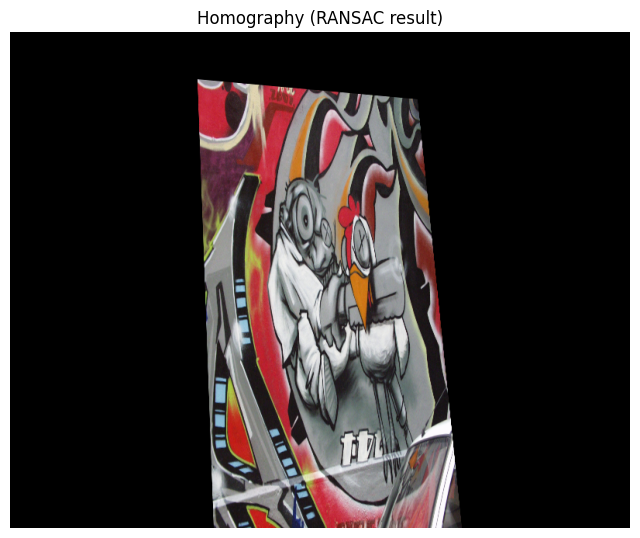
\includegraphics[width=0.95\columnwidth]{fig/4.2.png}
    \caption{Visualization of inlier matches and estimated homography (Q4.2).}
    \label{fig:q4_2}
\end{figure}

\noindent\textit{Note: The homography estimation process (Htansform) may need to be run several times to obtain a correct or optimal transformation, due to the random sampling nature of RANSAC.}

\subsection*{4.3 Final Image Stitching}
After estimating the homography, we warp \texttt{img1.ppm} onto \texttt{img5.ppm} to create a stitched panorama. The following code performs the warping and blending:
\begin{lstlisting}[language=Python, style=mystyle]
final_transformed_image = transform.warp(img1, htrans.inverse)
final_transformed_image = (final_transformed_image * 255).astype(np.uint8)
mask = (final_transformed_image == 0)
stitched_image = mask * img5 + final_transformed_image

plt.figure(figsize = (10, 10))
plt.imshow(stitched_image)
plt.title("Stitched Image")
plt.axis('off')
plt.tight_layout()
# Optionally save:
# from matplotlib import image as mpimg
# mpimg.imsave('fig/stitched_img1_on_img5.png', stitched_image)
\end{lstlisting}

\vspace{0.3em}
\noindent\textbf{Projective Transform Matrix Used:}
\begin{equation*}
\mathbf{H} =
\begin{bmatrix}
 0.4546 & -0.0195 & 241.586 \\
 0.0488 & 0.8912 & 62.064 \\
 0.00019 & -0.00022 & 1.0
\end{bmatrix}
\end{equation*}
\begin{figure}[H]
    \centering
    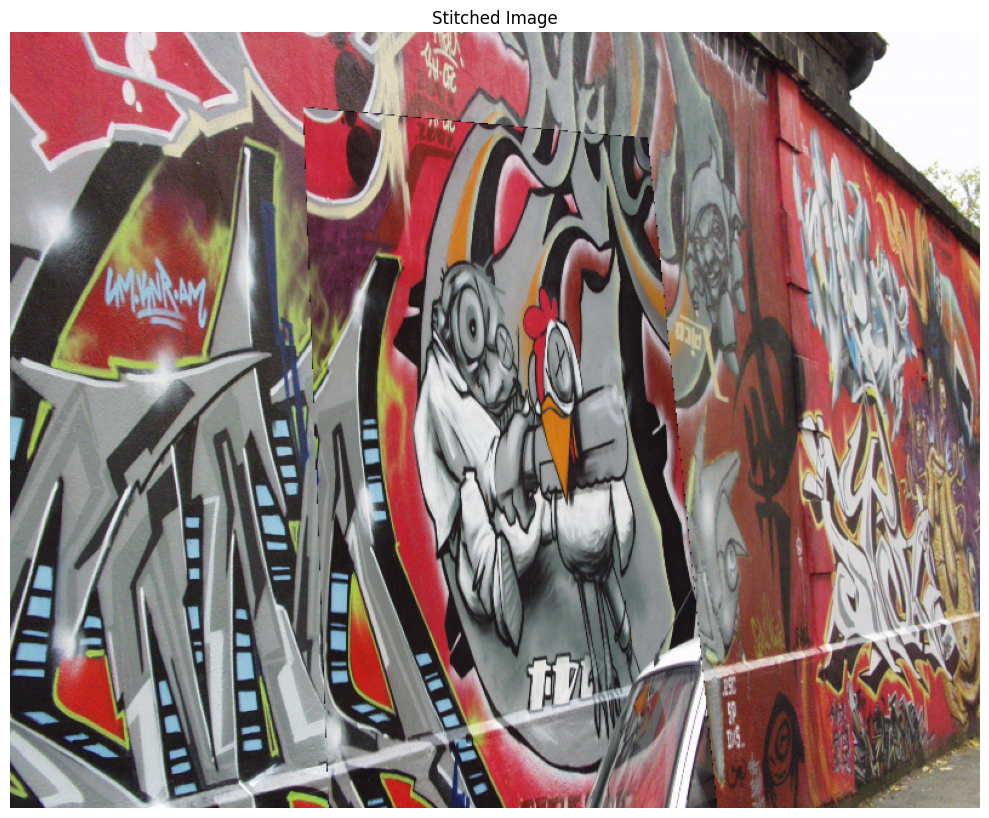
\includegraphics[width=0.95\columnwidth]{fig/4.3.png}
    \caption{Q4.3: Stitched result of \texttt{img1.ppm} onto \texttt{img5.ppm} using the estimated homography.}
    \label{fig:q4_3}
\end{figure}

\noindent\textit{The final stitched image demonstrates the effectiveness of SIFT feature matching and RANSAC-based homography estimation for image mosaicing.}

\end{document}
